\chapter{Energy Harvesting in IoT}
In general, finite battery capacity calls for a tradeoff between performance and lifetime of IoT devices, which is a major challenge in the IoT domain. Energy harvesting is a promising solution to this challenge, as it can provide a continuous and sustainable energy source for IoT devices. In this chapter, we provide an overview of energy harvesting in IoT, including the energy sources, energy harvesting techniques, and the challenges and opportunities in this area.

\section{Introduction and definitions}
Energy harvesting converts energy from one form to another.
If the harvested energy source
is large and periodically/continuously available, a device can last ``forever''.
This approach also allows to tune the device parameters for a better performance, since it removes the constraint of lifetime.

Note that the energy production varies with time and on environmental conditions; 
this is an aspect typically out of the control of the designer.

\begin{definition}[Energy Source]
   {\ns Source of energy to be harvested
   \note{Sun, wind, etc\dots}}
\end{definition}

\begin{definition}
   [Harvesting source] 
   Any available harvesting technology, (solar cells, wind turbines, piezo-electric harvesters etc\dots) that extracts energy from the environment.
\end{definition}

\begin{definition}
   [Load]
   Consumption of energy in a device due to its activities
   \begin{itemize}
      \item A device has many subsystems
      (processor/memory, radio, storage,
      transducers/ADC), each with its own states and
      consumption
      \item The load varies over time:
      depends on the specific activities the device is
      executing at a time
   \end{itemize}
\end{definition}

\begin{definition}
   [Harvesting System]
      A system that supports a variable load from a variable energy-harvesting source, also when the instantaneous power supply levels from the harvesting source do not match the load.
\end{definition}

\subsection{Takeaway}
In theory, there are two main approaches:
{\ns\begin{enumerate}
   \item \textbf{adapt the load} to the actual energy supply
   \item use an \textbf{energy buffer}
   \note{i.e. a rechargeable battery or a
   supercapacitor}
\end{enumerate}}

However, in practice \ul{neither of these two approaches may be sufficient}, since the load cannot be reduced arbirarily, and the buffer is not ideal (no infinite storage and eventually energy leaks).
\newpage
\section{Harvesting Architectures}
\subsection{Harvest-use}
\begin{paracol}{2}

   In this architecture energy is harvested just-in-time for use.\\
   The power output has to be above the minimum operating point (else the device turns OFF), 
   but note that this might leads abrupt variations to cause the device to oscillate between ON and OFF states.
   
   The problem is that a device may suffer from ``Alzheimer's disease'', i.e. it forgets what it was doing before turning OFF, since the content of the RAM is lost.
   \note{This is an issue currently being addressed by researchers.}
   
   \switchcolumn
   
   \begin{figure}[htbp]
      \centering
      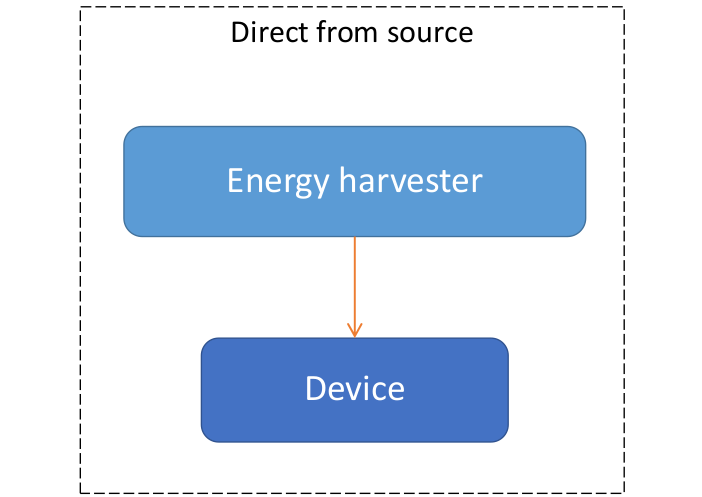
\includegraphics[width=0.45\columnwidth]{images/harvestuse1.png}
      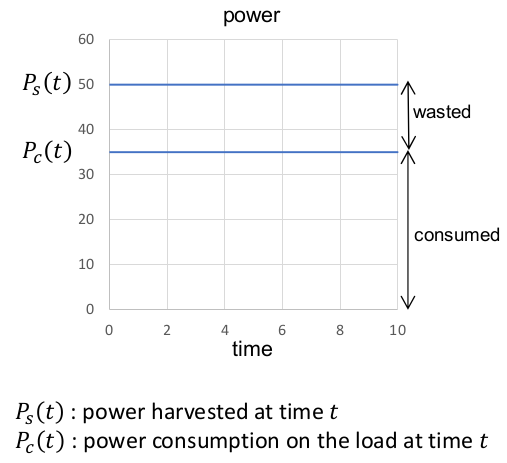
\includegraphics[width=0.45\columnwidth]{images/harvestuse2.png}
      \caption{Harvest use schema}
      \label{fig:harvestuse}
   \end{figure}
\end{paracol}

The energy harvested, but not required by the device functioning is \textbf{wasted}.

\subsection{Harvest-store-use}
\begin{paracol}{2}
   \colfill
   Energy is harvested whenever
   possible and stored for future
   use.\\
   Residual energy is stored and it
   is used later when either there
   are no harvesting opportunities
   or the device tasks require more
   energy.
   \colfill
   \switchcolumn
   \begin{figure}[htbp]
      \centering
      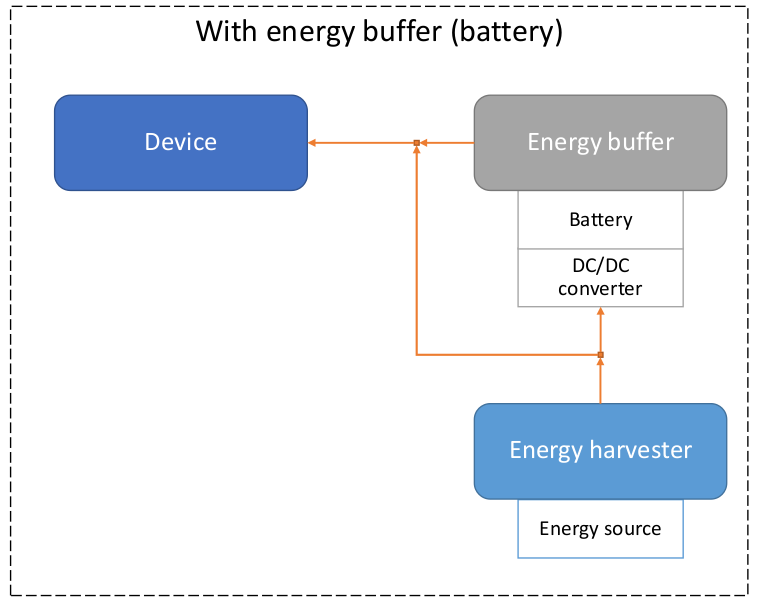
\includegraphics{images/harveststoreuse1.png}
      \caption{Harvest-store-use schema}
      \label{fig:harveststoreuse1}
   \end{figure}
\end{paracol}

\begin{paracol}{2}
   
   We assume for the moment that the energy buffer is ideal, i.e. it can store an infinite amount of energy, it does not leak, and has a charging efficiency $\eta = 1$.\\
   Under such assumptions the device can operate at any time if, for every time interval $(0,T]$
   \begin{align*}
      P_s(t) & \quad & \textit{power harvested at time t}\\
      P_c(t) & \quad & \textit{power consumed on the load at time t}\\
      B_0 & \quad & \textit{initial energy in the buffer}
   \end{align*}
   \[
      \int_0^T P_c(t)dt \leq \int_0^T P_s(t)dt + B_0 \quad \forall T \in (0, \infty)
      \]
      
      \switchcolumn
      \begin{figure}[htbp]
         \centering
         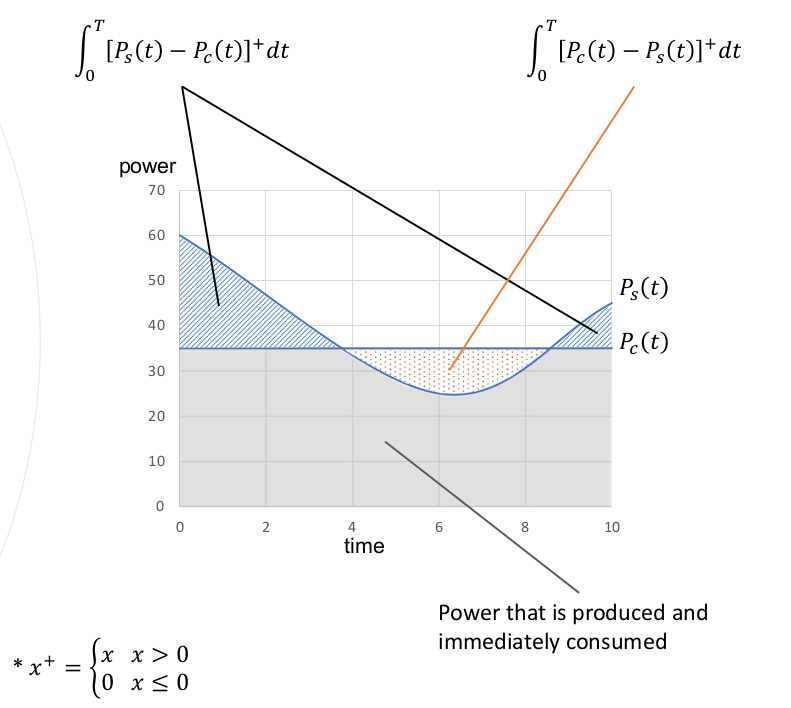
\includegraphics{images/harveststoreuse2.png}
         \caption{Harvest-store-use modeling schema}
         \label{fig:harveststoreuse2}
      \end{figure}
   \end{paracol}

\subsection{Harvest-store-use with a non-ideal buffer}
We need to introduce other symbols
\begin{align*}
   B_{max} & \quad & \textit{maximum battery capacity (energy buffer size)}\\
   B_{t} & \quad & \textit{battery charge at time t}\\
   P_{leak}(t) & \quad & \textit{be the leakage power of the battery at time t}\\
   \eta < 1 & \quad & \textit{be the charging efficiency of the battery}\\
   P_s(t) & \quad & \textit{power harvested at time t}\\
   P_c(t) & \quad & \textit{load at time t}\\
   B_0 & \quad & \textit{initial charge of the buffer}\\
   x^+ = \begin{cases}
      x & \text{if } x > 0\\
      0 & \text{otherwise}
   \end{cases} 
   & \quad & x^+\textit{is a ``rectifier function''}
\end{align*}

\[
   B_T = B_0 + \eta\int_0^T[P_s(t) - P_c(t)]^+dt - \int_0^T[P_c(t) - P_s(t)]^+dt - \int_0^T P_{leak}(t)dt   \quad \forall T \in (0, \infty]
\]

\subsection{Exercise}
\begin{figure}[htbp]
   \centering
   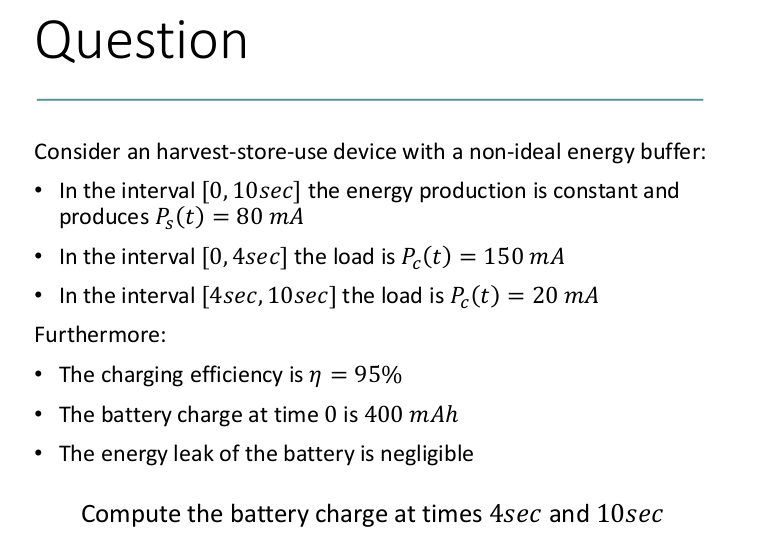
\includegraphics{images/harveststoreuse_question.png}
   \label{fig:harveststoreuse_question}
\end{figure}
\begin{equation}   
\begin{split}
   \textit{Conversion from mAs to mAh} & 3600 mAs = 1 mAh \\
   \\
   400mAh + \hcancel[red]{0.95\times (80-150=-70)\times 4} - 4\times (150-80=70)mAs\\
   400mAh - 280mAs/3600 = 399.92mAh\\
   \textit{\ul{Battery charge at time 4 sec}} = 399.92mAh\\
   \\
   399.92mAh+ 0.95\times (80-20=60)\times 6/3600mAh - \hcancel[red]{6\times (20-60=-40)}\\
   \textit{\ul{Battery charge at time 10 sec}} = 400.02mAh 
\end{split}
\end{equation}

\section{Energy sources classification}
\begin{itemize}
   \item \textbf{Fully controllable} energy sources can provide harvestable energy whenever required.
   \note{Example self-power flashlights: the user may shake to generate energy whenever needed}
   \item \textbf{Partially controllable} energy sources may be influenced by the system design, but the result may not be deterministic
   \note{e.g. RF energy source installed in a room and RFID’s may extract energy from it. However,
   the energy produced at a node depends on RF propagation in the room that cannot be fully
   controlled}
   \item \textbf{Non-controllable} energy sources cannot be activated on demand.
   In these cases the energy must be harvested whenever available.
   \note{e.g. wind, sun, etc\dots}
   \begin{itemize}
      \item \textbf{Predictable} energy sources are those for which there exist reliable models
      that forecast the energy availability.
      \note{e.g. Sun cannot be controlled but it can be predicted (to some extent).
      Day/night production, summer/winter, weather forecasts, \dots}
      \item \textbf{Unpredictable}
      energy sources are those for which there not exist reliable models that forecast the energy availability
      \note{e.g. vibration due to sources for which there are no models available (earthquakes etc\dots)}
   \end{itemize}
\end{itemize}

\begin{figure}[htbp]
   \centering
   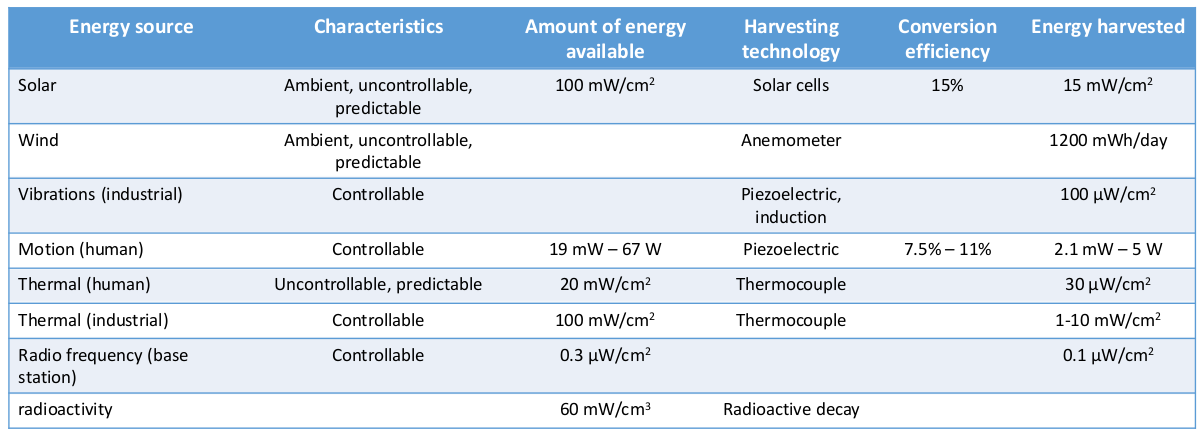
\includegraphics{images/energysources.png}
   \caption{Energy sources summary}
   \label{fig:energysources}
\end{figure}
\note{Fun fact: the efficiency of the plants' photosynthesis is around $10-15\%$}

\section{Harvesting sources}
\subsection{Radio Frequency (RF) energy}
When electromagnetic radio frequency (RF) field passes through an
antenna coil, an AC voltage is generated across the coil.

A passive RF tag powers itself by using RF energy transmitted to it;
active RF tags instead have their own battery.

RFIDs are used to identify, locate and track people, assets and animals:
An RFID reader queries an RFID tag by sending RF signal, and the RFID tag is entirely powered by the energy harvested by the antenna coil.
This energy is just sufficient to send back a reply.

\subsection{Piezo-electric energy}
Use mechanical force to deform a piezo-electric material,
which results in an electric potential difference.
\begin{itemize}
   \item Piezo-electric \textit{films}: \texttt{PVDF} (PolyVinylidene Fluoride)
   \item Piezo-electric \textit{ceramic}: \texttt{PZT} (Lead Zirconate Titanate)
   \item[] PVDF is more flexible than PZT
\end{itemize}

\subsection{Wind turbines}
There are some wind turbines for IoT applications, which are:
\begin{itemize}
   \item Small size
   \item Low height
   \item Operative range with weak winds
\end{itemize}

\begin{paracol}{2}
   When reading articles about energy harvesting, it is common to encounter diagrams like the one in Fig. \ref{fig:windturbines}. 
   Different Load resistances provide different efficiency, meaning that the energy produced does not depend only on the wind speed, but also on the load resistance, and does not decrease \textit{linearly}.
   \switchcolumn
   \begin{figure}[htbp]
      \centering
      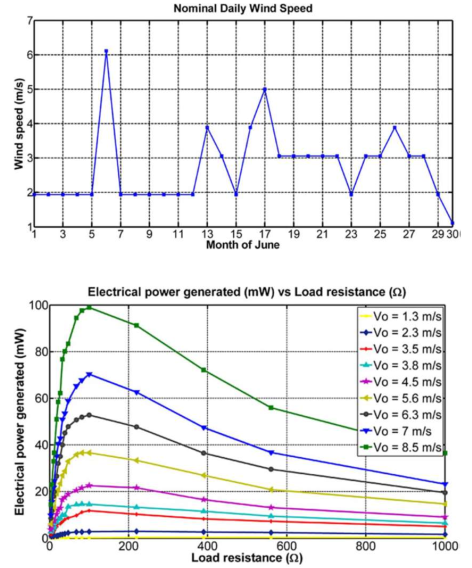
\includegraphics{images/windturbines.png}
      \caption{Wind turbines energy production diagram}
      \label{fig:windturbines}
   \end{figure}
\end{paracol}

\subsection{Solar energy}
\begin{paracol}{2}
   \colfill
   The energy production of a panel depends on several factors:
   \begin{itemize}
      \item \textbf{Solar radiation}
      {\ns\note{Depends on the angle drawn by the Sun with, respect to the vertical axis of the Earth surface,that depends on the geographical position of the panel, and on the day in the year; besides it also depends on the weather conditions.}}
      \item \textbf{Size of the panel}
      \item \textbf{Charging efficiency}
   \end{itemize}
   The typical countermeasure to such variations is to \textit{oversize} the harvesting subsystem and battery capacity to match with the worst conditions. 
   \colfill
   \switchcolumn
   \begin{figure}[htbp]
      \centering
      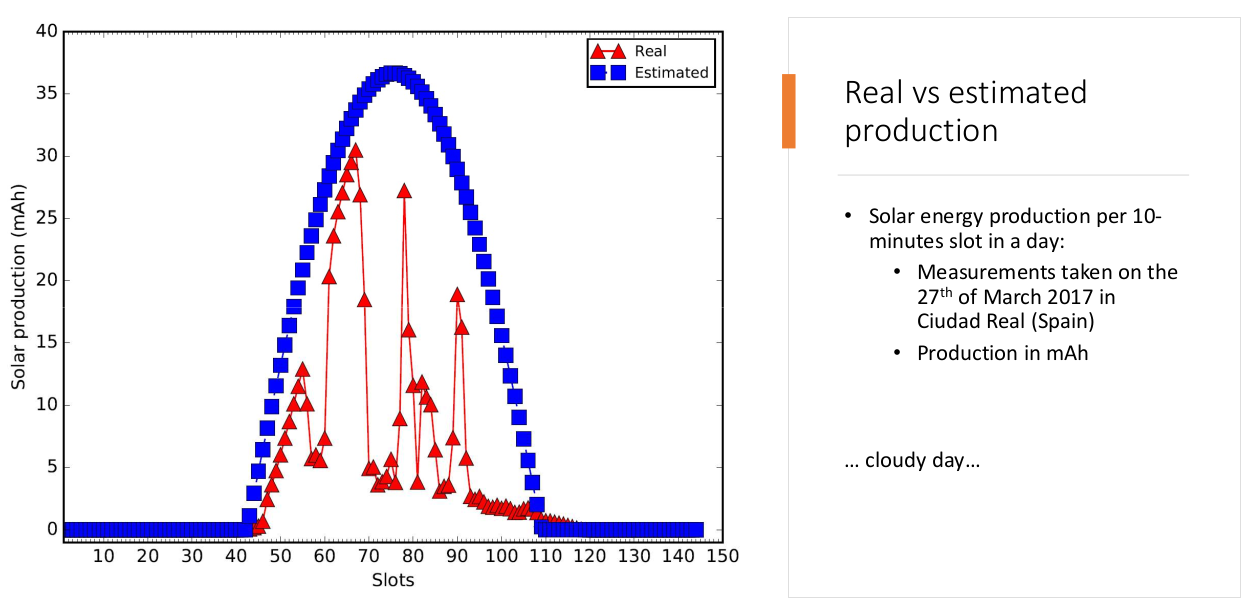
\includegraphics{images/solarharvesting.png}
      \label{fig:solarharvesting.png}
   \end{figure}
\end{paracol}


\subsection{Considerations}
\begin{center}
   \textit{\ul{Energy harvesting does not mean that a device is always operational!}}
\end{center}

If the device is harvesting solar and wind energy, the residual battery may not last for a whole windless night, so the device may turn off during the night and back on in the morning. 

\section{Storage technologies}
\begin{figure}[htbp]
   \centering
   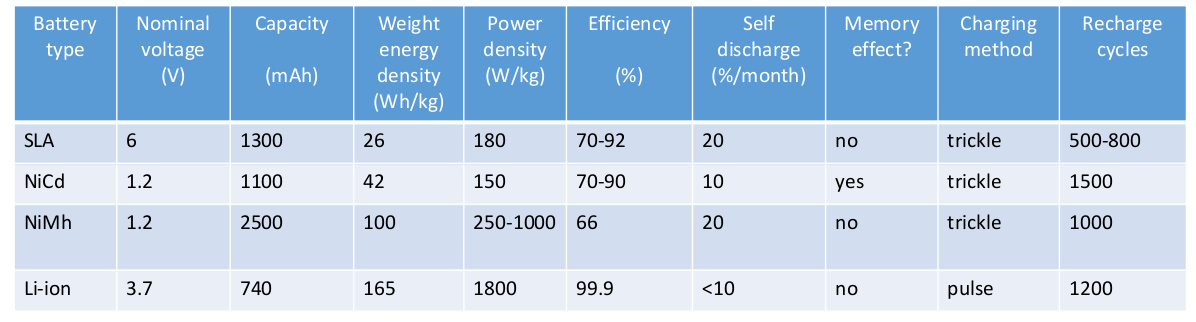
\includegraphics{images/batterycomparison.png}
   \caption{Comparison amongst different battery cell types}
   \label{fig:batterycomparison}
\end{figure}
There are for main battery cell types, listed below and compared in Fig. \ref{fig:batterycomparison}:
\begin{enumerate}
   \item Sealed Lead Acid (\texttt{SLA})
   \item Nickel Cadmium (\texttt{NiCd})
   \item Nickel Metal Hydride (\texttt{NiMH})
   \item Lithium Ion (\texttt{Li-ion})
\end{enumerate}

\begin{paracol}{2}
   \colfill
   \textbf{Supercapacitors} are a new highly efficient technology, but with high discharge rate and low power density.
   They can be used to buffer energy if energy source is jittery: when no-load, allows to charge at the same rate of discharge to keep the capacitor at full charge level (\textit{trickle charging}). 
   \colfill
   \switchcolumn
   \begin{figure}[htbp]
      \centering
      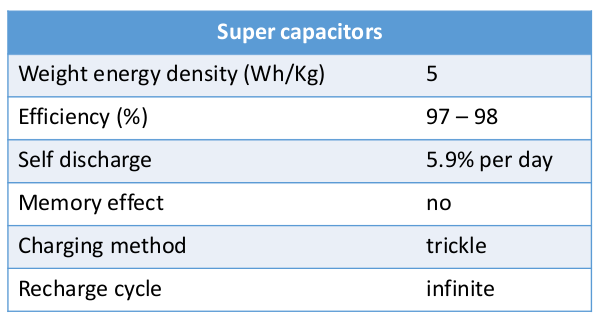
\includegraphics{images/supercacitors.png}
      \caption{Supercapacitors specs}
      \label{fig:supercacitors}
   \end{figure}
\end{paracol}

\section{Measuring discharge}
\begin{figure}[htbp]
   \centering
   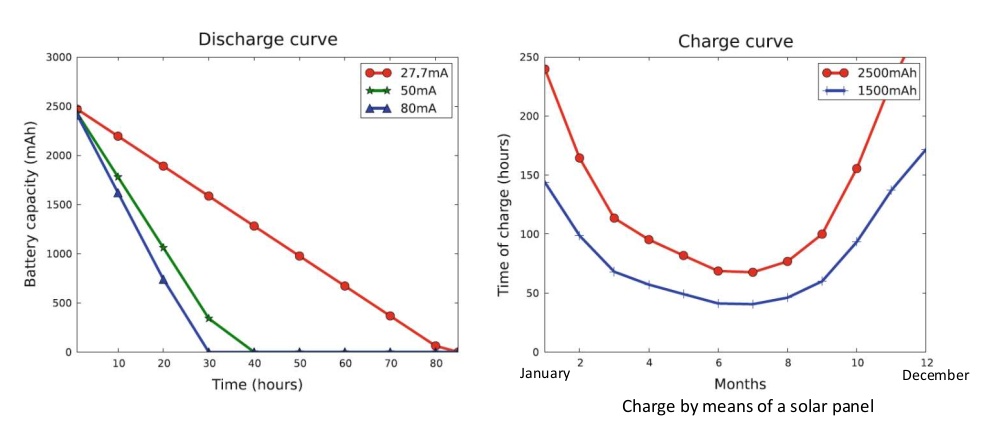
\includegraphics{images/charge_discharge.png}
   \label{fig:chargedischarge}
\end{figure}

In order to decide which storage to adopt, it is crucial to measure its discharge, to properly choose a solution which fits the requirements.

\framed{
   We may measure the battery discharge using mathematical theorems and equations:\\
   assume ---an \textit{ideal energy buffer} and that--- we have a method for measuring the battery
   charge $E_b(t)$ at time $t$, and that the power consumption $p_c(t)$ in a time frame $[t_1,t_2]$ is known,
   then the energy $E_e$ produced in the same time frame is
   given by the following equation
   \[
      E_e = \left[\int_{t_1}^{t_2}p_c(t)dt + E_b(t_2) - E_b(t_1)\right]^+   
      \]
}
      
A better way is to \ul{use electronic circuits to measure the current flowing out} of the harvesting source and its voltage.
Using a $d$-bits ADC and assuming minimum and maximum voltage values ($v_{min}$ and $v_{max}$, corresponding to $x_{min}$ and $x_{max}$, the "$d$-bits" values read by the ADC) the battery charge may be obtained with this equation
\[B = B_{min} + \frac{B_{max} - B_{min}}{x_{max} - x_{min}}(x - x_{min})\]

\section{Modulating the load}

An IoT device has several components, each
characterized by a power consumption (cost)
per unit of time,
in fact components can be turned on/off by the
processor when not in use, and even the processor can be put in low-power mode.

\textit{Load modulation} means reducing the amount of work
to reduce the energy consumption.
\note{
   For example, a device may vary the sampling frequency of its sensor:
   \parskip = \baselineskip
   \begin{itemize}
   \item High sampling frequency implies high
   energy cost (but also high utility)
   \item Low sampling frequency implies low
   energy cost and low utility
\end{itemize}
}

Earlier on the goal was to maximize the device lifetime, but nowdays the standard approach is to obtain \ul{\textbf{energy neutrality},which is the ability of a device to keep the desired performance level ``forever''.} 
\newpage

\section{Energy neutrality}
\begin{enumerate}
   \item \textbf{Energy-Neutral Operation}:\\
   \textit{How to operate such that, in any give time frame,
   the energy used is always less than the energy harvested?}
   \item \textbf{Maximum Performance:}\\
   While ensuring energy-neutral operation, what is the maximum performance level that can be supported in a given harvesting environment?
\end{enumerate}

The key elements are
\begin{itemize}
   \item The amount of harvested energy from (each) source
   \item The current charge of the battery
   \item The power consumption of the device (the load), which is modulated to ensure energy neutrality
   \item The future energy production estimation
   \begin{itemize}
      \item By means of weather forecasts or other
      methods
      \item Subject to errors
      \item Usually under pessimistic assumptions: errors maximized and expected production minimized
   \end{itemize}
\end{itemize}

\begin{figure}[htbp]
   \centering
   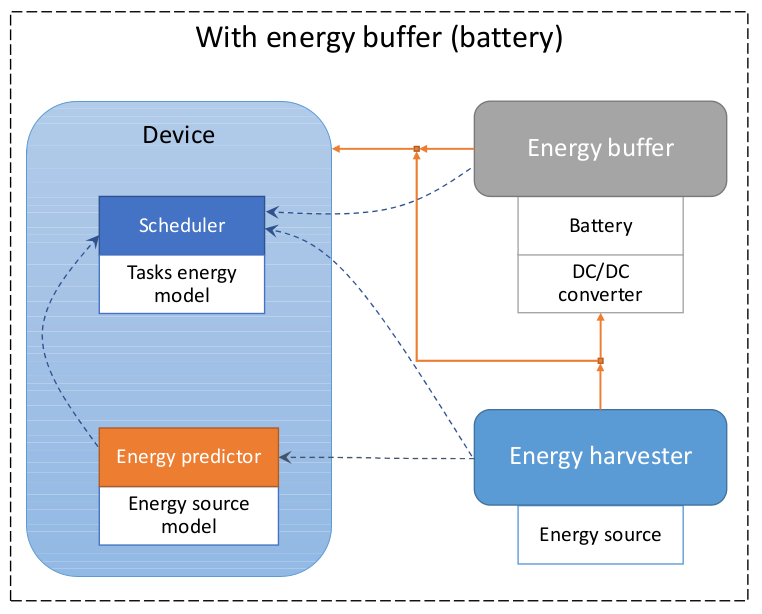
\includegraphics{images/harveststoreuse_revisited.png}
   \caption{Revisited harvest-store-use diagram}
   \label{fig:harveststoreuse_revisited}
   Energy is stored for ``future use'' and is used later when either there are no harvesting opportunities, or the sensor tasks require more energy
\end{figure}

\subsection{Kansal's algorithm for Power Management}
Kansal considers the case of \ul{\textit{predictable} but \textit{uncontrollable} sources}.

The objectives are three:
{\ns
\begin{enumerate}
   \item keep the system \textbf{energy neutral}
   \item ensure the system \textbf{never fails} due to energy depletion
   \item maximize the node's \textbf{performance}
\end{enumerate}}
and the approach to do so is to take current end expected battery charge into account and dynamically tune the device’s performance (and thus the load),
so that the device \textit{neither} operates below minimum performance levels nor switches OFF before the next recharge cycle.

\newpage

\begin{paracol}{2}
   \begin{figure}[htbp]
      \centering
      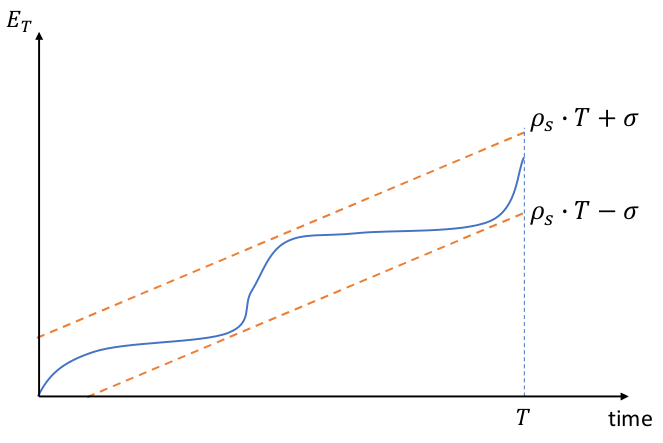
\includegraphics{images/kansal_1.png}
      \caption{Kansal $1^{st}$ condition: \textit{energy production}}
      \label{fig:kansal_1}
   \end{figure}
   \switchcolumn
   \colfill
   \[E_T = \int_{T}P_S(t)dt\]
   $E_T$ is the amount of energy produced in a $[0,T]$ interval.
   By looking at the graph, we note/assume that for some $\rho_S,\sigma \in \mathbb{R}$
   \[\rho_S T - \sigma < E_T \leq \rho_S T + \sigma\] 
   \colfill
\end{paracol}

\begin{paracol}{2}
   \begin{figure}[htbp]
      \centering
      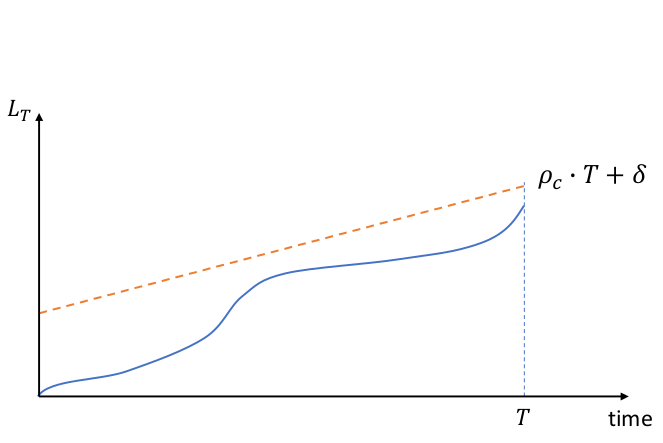
\includegraphics{images/kansal_2.png}
      \caption{Kansal $2^{nd}$ condition: \textit{load}}
      \label{fig:kansal_2}
   \end{figure}
   \switchcolumn
   \colfill
   \[L_T = \int_{T}P_C(t)dt\]
   $L_T$ is the amount of energy consumed in a $[0,T]$ interval.
   for some $\rho_S,\phi \in \mathbb{R}$
   \[0 < L_T \leq \rho_C T + \Sigma\] 
   \colfill
\end{paracol}

\framedt{Kansal's theorem}{
   if the previous assumptions on $E_T$ and $L_T$ \textit{hold},
   and the energy buffer is characterized by charging efficiency $\eta$ and leakage $\rho_{leak}$,
   then \ul{a sufficient condition for energy neutrality of the system} is:

   % \begin{figure}[htbp]
   \begin{center}
      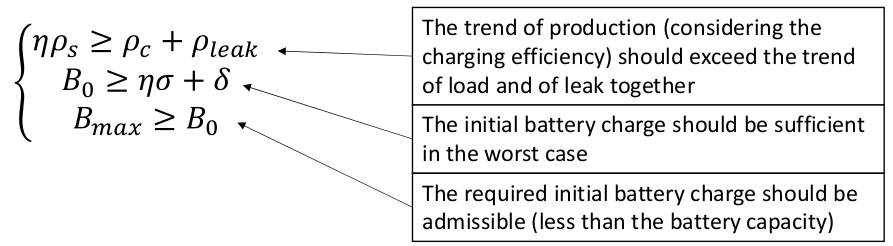
\includegraphics{images/kansal_theorem.png}
   \end{center}
   %    \label{fig:kansal_theorem}
   % \end{figure}
}

Kansal's model of utility and duty cycle enables a modulation of the load on the energy harvesting device.
Consider a system designed to detect the presence of intruders in a room.
\begin{itemize}
   \item The minimum and the maximum duty cycles imply a range of possible sampling frequencies
   \item The higher the frequency the better the ability to detect intruders and the higher is thus the
   utility
   \item The lower the frequency the lower is the ability to detect the intruders and thus the utility
   \item Below $dc_{min}$ the detection ability is impaired
   \item Above $dc_{max}$ it is useless to sample (the intruder is not that fast\dots)
\end{itemize}

{\ns This leads to an \textit{optimization problem} where:
\begin{itemize}
   \item The \textit{production varies} over time (uncontrolled), but it is \textit{predictable} (by assumption)
   \item The \textit{load varies} over time according to the duty cycle (controlled)
   \item The battery \textit{charge varies} over time accordingly
   \item[] \note{The battery charge variation may be computed, using the ---controlled--- load and the forecasted energy production}
\end{itemize}}
\framed{
   Since the energy source is \textit{predictable} we have to find the load so that the \textit{system is energy \textbf{neutral}} and the overall \textit{\textbf{utility} is maximized}
}
\nl

Kansal's approach to assign a duty cycle at each time slot (assuming time is slotted), does not require the knowledge of the future production\footnote{However it may be available in some cases, such as weather forecasting}, but just an \textit{estimation} based on previous observations, an it builds the cycle over three components:
\begin{enumerate}
   \item forecasts future power production based on past power production, using a \texttt{EWMA} (Exponentially Weighted Moving Average) filter\footnote{i.e. assumes the future production to be similar to the past day}
   \begin{equation}
      \tilde{p}^{j+1}_S(i) = \alpha \cdot\tilde{p}^j_S(i) + (1-\alpha)\cdot\tilde{p}^j_S(i)
   \end{equation}
   \item uses a simple polynomial-time algorithm (suitable for low-power processors) to solve the
   optimization problem
   \item performs a reoptimization (dynamic adaptation) if the actual power production deviates
   significantly from the expected one
\end{enumerate}

\framed{
   $k$ number of time slots\\
   $B(i)$ battery charge at the beginning of slot $i$\\
   $B(k+1)$ battery level at the end of slot $k$ (i.e. at the end of the day)
   \nl
   
   Based on the expected power production $\tilde{p}_S(i)$ at each slot $i \in [1,k]$, the algorithm assigns a duty cycle $dc(i)$ and hence a utility $u(i)$to each slot $i$,
   while requiring that $B(k+1)\geq B(1)$ i.e. that the system must be \textit{energy neutral}.
}


\textit{\ul{What about the number of time slots $k$?}} There is not a fixed number and there is not a method to determine the best one; three considerations may be done in regards to it:

\begin{enumerate}
   \item Too small implies a simpler model, but higher risk of error. Too large implies a possibly (not necessarily)more accurate model, but higher computational cost
   \item If time slots are too small ($k$ is large) the signal output may present too many oscillations
   \note{Consider a device which every minute changes the sample rate: this may lead to a lot of oscillations in the signal output, resulting in more complicate data analysis}
   \item If time slots are too small, you may not be able to properly feed the estimation model, e.g. 1-minute slotting may not be significant to estimate the production of a solar panel
\end{enumerate}

\section{Task-based model for Energy Neutrality}
Usually, an application for an IoT device implements 4 steps in a cycle, each one with a potentially different implementation:
\begin{enumerate}
   \item Sensing
   \item Storing
   \item Processing
   \item Transmitting
\end{enumerate}

Different implementations may imply a different
behaviour of the server (either in the gateway or in the
cloud).
Even though the system functionality does not change, the implementation may change indeed.
\begin{itemize}
   \item 
   Example 1:\\
   If the application process all data and transmits only the
   results, the server may just store the received data.
   \item Example 2:\\
   If the application just transmits all the sensed data, then the server has to process and then store the
   data.
\end{itemize}


   \begin{figure}[htbp]
      \centering
      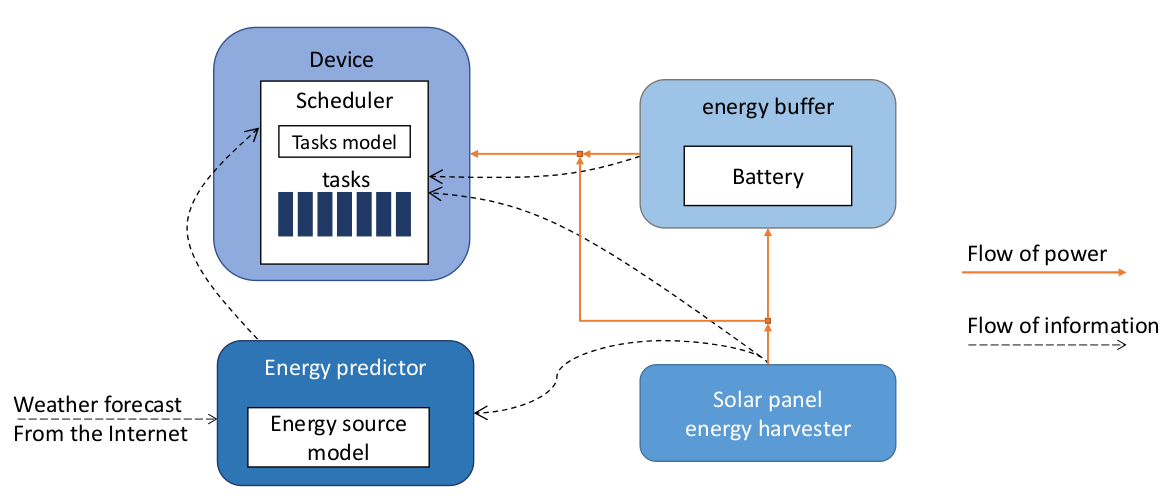
\includegraphics{images/taskmodel.png}
      \caption{Task based model architecture}
      \label{fig:taskmodel}
   \end{figure}

   We call \ul{\textbf{task} an implementation of the application in the IoT device.}
   We may achieve \textit{load modulation} by scheduling the tasks in execution; clearly, the server needs to know which task is running to behave accordingly.
   
   To each task we may associate a \textit{power consumption} and a \textit{utility}, allowing a dedicated \textit{task scheduler} component to properly choose the task to run in each \textbf{time slot}.
   
   \note{Kansal's time slotting goes nicely along with this architecture}


The scheduler must solve an \textbf{optimization problem} by means of linear programming, which is to maximize the utility of the tasks assigned to the slots:
\begin{equation}
   max \sum_{i=1}^{k}u(i) \sum_{j=0}^{n}x_{i,j}\cdot u_{j}
\end{equation}

Given:
\begin{align}
   \sum_{j=1}^{n}x_{i,j}=1 \forall i \in [1,k] & \quad & \textit{exactly one task per slot}\\
   B(1) \leq B(k+1) & \quad & \textit{energy neutrality}\\
   B_{min} \leq B(i) \forall i \in [1,k] & \quad & \textit{Battery may never go below the minimum}\\
   B(i+1) = min\left\{B_{max}, B(i) + \eta\cdot p_S^+(i) - p_C^-(i) \forall i \in [1,k]\right\} & \quad & \begin{aligned}\textit{$i^{th}$ slot charge depends on initial charge,} \\ \textit{production, and consumption in the slot}\end{aligned}
\end{align}

The described problem may be reduced to the famous \textit{knapsack problem}, which --sadly--- is \textbf{NP-hard}, thus hardly solvable for most commodity PCs, let alone for IoT devices.

The knapsack problem is solvable by means of a \textit{dynamic programming} approach, exploiting is a \textit{polynomial-time} algorithm.\\
Assuming that the system state is defined by $(i,b)$, where
\begin{itemize}
   \item $i$ is the time slot up to which the system is optimized
   \item $b$ is the battery charge at the beginning of the slot
\end{itemize}
Then the optimal utility $opt(i,b)$ can be computed exploiting a backware recursive rule:
\begin{align}
   opt(k,b) = max_{j=1,\dots,n} \left\{u_j : b + \eta\cdot p_S^+(k) - p_C^-(k) \geq B(1)\right\}\\
   opt(i,b) = max_{j=1,\dots,n} \left\{u_j : opt\left(i+1, B^j(i+1)\right):B^j(i+1) \geq B_{min}\right\}
\end{align}
\note{
   \begin{itemize}
      \item 
      Where in $opt(k,b)$ results from assuming task j is assigned to slot k
      \item Where $B (i+1)$ is the residual battery at the end of slot $i$ if task $T$ is assigned to that slot
   \end{itemize}
   }